\chapter{Historical Models of Image Generation}

In this chapter, I will explore three key generative modeling techniques: Noise Contrastive Estimation (NCE), Variational Autoencoders (VAEs), and Diffusion Models. These models represent significant milestones in the development of generative modeling approaches, each with its unique advantages and limitations. 

\section{Noise Contrastive Estimation}

\subsection{Principles of NCE}

Noise Contrastive Estimation (NCE) was introduced in 2010 by Gutmann and Hyvärinen as a method for estimating parameters of unnormalized probabilistic models. It offers an alternative to Maximum Likelihood Estimation (MLE), which can be computationally expensive for large-scale models. NCE reframes the complex task of normalizing probability distributions into a more tractable binary classification problem \citep{10.48550/arxiv.1711.00658}.

In traditional MLE, training models for unnormalized probability distributions involves calculating the partition function, which is often computationally intractable. NCE avoids this issue by introducing noise samples drawn from a known distribution. The model is then trained to discriminate between real data samples and noise samples. Specifically, the model assigns higher probabilities to real data and lower probabilities to noise, indirectly learning the data distribution without requiring normalization \citep{10.48550/arxiv.2110.11271}.

\subsubsection{NCE Architecture and Process}

At the core of Noise Contrastive Estimation is the idea of reframing MLE as a binary classification task. In traditional MLE, training models for unnormalized probability distributions involves calculating the partition function, which is computationally intractable in large-scale models. NCE avoids this issue by introducing noise samples drawn from a known distribution. The model is then trained to discriminate between real data samples and noise samples. Specifically, the model assigns higher probabilities to real data and lower probabilities to noise, thus indirectly learning the data distribution without requiring normalization \citep{10.48550/arxiv.2110.11271}.

The objective function in NCE is derived by reformulating the likelihood of a data point \( x \) as the probability that it is real, rather than noise. Given a dataset \( D \) with real samples \( x_i \) and noise samples \( x_j \), the probability \( P(y = 1 | x) \), where \( y = 1 \) indicates a real sample and \( y = 0 \) indicates a noise sample, is given by:

\begin{equation}
P(y = 1 | x) = \frac{p_{\theta}(x)}{p_{\theta}(x) + k p_{\text{noise}}(x)}
\end{equation}

Where:
\begin{itemize}
    \item \( p_{\theta}(x) \) is the unnormalized model probability assigned to the data sample \( x \).
    \item \( p_{\text{noise}}(x) \) is the known probability of the noise sample.
    \item \( k \) is the ratio of noise samples to real samples.
\end{itemize}

The corresponding probability for a noise sample is given by:

\begin{equation}
P(y = 0 | x) = \frac{k p_{\text{noise}}(x)}{p_{\theta}(x) + k p_{\text{noise}}(x)}
\end{equation}

The NCE objective then maximizes the log-probabilities of real data and noise data being correctly classified:

\begin{equation}
\mathcal{L}_{NCE} = \sum_{i=1}^{N} \left[ \log P(y=1 | x_i) + \sum_{j=1}^{k} \log P(y=0 | x_j) \right]
\end{equation}

This reformulation circumvents the need to compute the partition function, which makes NCE particularly effective for large-scale models.

As shown in Figure~\ref{fig:NCE_structure}, the architecture of a typical NCE model includes an input layer, hidden layer, and output layer. The input layer takes in data samples (both real and noise), while the hidden layer learns a representation of these samples. The output layer, modeled as a binary classification task, outputs is a probabilities indicating whether a given sample is real or noise.

\begin{figure}[H]
    \centering
    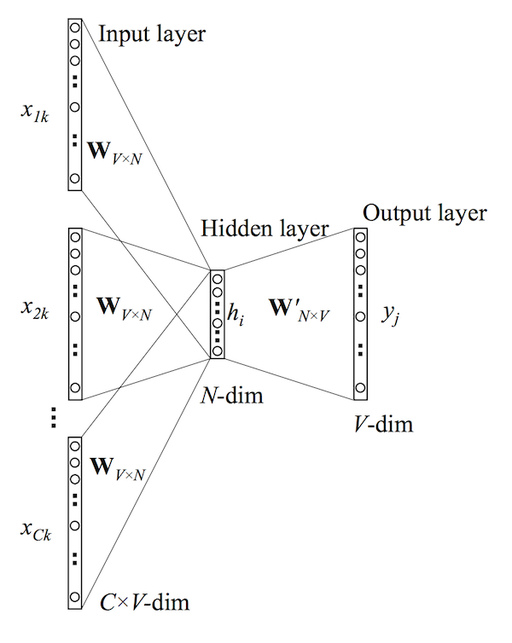
\includegraphics[width=0.9\textwidth]{./Images/NCE_structure.jpg}
    \caption{NCE architecture showing the input, hidden, and output layers.}
    \label{fig:NCE_structure}
\end{figure}

\begin{itemize}
    \item \textbf{Data and Noise Samples}: NCE introduces noise samples from a known distribution to compare with the actual data. These noise samples serve as negative examples in the binary classification task, while real data serves as positive examples \citep{10.48550/arxiv.1711.00658}.
    \item \textbf{Binary Classification}: The task of differentiating between real and noise samples is formalized as a binary classification problem, which can be optimized using standard logistic regression techniques \citep{10.18653/v1/e17-2003}.
\end{itemize}

By transforming the estimation problem in this way, NCE simplifies the computation and circumvents the need for calculating the partition function, which is often the bottleneck in MLE for large-scale models.

\subsection{Comparison with GANs}

Noise Contrastive Estimation (NCE) and Generative Adversarial Networks (GANs) are both prominent techniques used in machine learning, but they differ significantly in their approach to model training and estimation.

\begin{itemize}
    \item \textbf{Training Stability}: One of the primary advantages of NCE over GANs is its stability during training. GANs often face challenges such as mode collapse and unstable training dynamics due to the adversarial nature of the training process, where the generator and discriminator are pitted against each other. In contrast, NCE transforms the model training process into a binary classification problem, which is generally more stable and can be optimized using standard logistic regression techniques \citep{10.18653/v1/e17-2003}.
    
    \item \textbf{Computational Efficiency}: GANs require training two models (generator and discriminator) simultaneously, which can lead to higher computational costs, particularly when tuning their interactions for optimal performance. NCE, on the other hand, simplifies the problem by reducing it to a comparison between real data and noise samples. This avoids the adversarial framework and allows for more efficient training, especially in large-scale models \citep{10.21437/interspeech.2016-1295}.
    
    \item \textbf{Handling Unnormalized Models}: NCE is particularly effective for training unnormalized probabilistic models, where the partition function is difficult or impossible to compute directly. GANs, however, are typically used for generating realistic data samples, and while they do not require explicit normalization, they do not address the estimation of unnormalized probabilistic models as NCE does \citep{10.48550/arxiv.2101.03288}.
    
    \item \textbf{Model Interpretability}: In NCE, the model explicitly learns to estimate the probability of data samples relative to noise, which can provide insights into the underlying data distribution. In contrast, GANs focus primarily on generating realistic samples, and their internal workings (particularly the latent space) can be less interpretable compared to NCE-based models.
    
    \item \textbf{Use in Language Models and Word Embeddings}: NCE is particularly advantageous in applications such as word embeddings and large-scale language models, where normalizing the likelihood function over a large vocabulary is computationally prohibitive. While GANs have been explored in text generation tasks, NCE's efficiency in handling large vocabulary sizes makes it a more suitable choice for these types of problems \citep{10.48550/arxiv.2101.03288}.
\end{itemize}

\subsection{Applications of NCE}

The utility of Noise Contrastive Estimation extends to various machine learning tasks. It is particularly effective in scenarios involving large datasets and unnormalized probabilistic models:
\begin{itemize}
    \item \textbf{Word Embeddings}: NCE is widely used in training word embeddings in natural language processing, where the vocabulary size makes exact normalization computationally infeasible.
    \item \textbf{Language Models}: In addition to word embeddings, NCE has been applied to train large-scale language models where traditional likelihood-based methods may become computationally prohibitive.
    \item \textbf{Energy-Based Models}: As mentioned earlier, NCE is effective in training energy-based models, where the partition function is challenging to compute directly.
\end{itemize}

By leveraging NCE, models can scale efficiently, making it a useful tool in a wide range of applications, from natural language processing to computer vision.

\subsection{Limitations of NCE}

While Noise Contrastive Estimation has proven to be an effective technique, it is not without limitations. One of the primary challenges lies in selecting an appropriate noise distribution. The choice of noise distribution is critical to the model's success; a poorly chosen noise distribution can lead to inaccurate parameter estimates and slower convergence during training \citep{10.48550/arxiv.2110.11271}.

\begin{itemize}
    \item \textbf{Noise Distribution Sensitivity}: NCE relies heavily on the assumption that the noise distribution is sufficiently different from the true data distribution. If the noise distribution is not carefully selected, the model may fail to accurately distinguish between real and noise samples \citep{10.48550/arxiv.2110.11271}.
    \item \textbf{Complex Data Distributions}: NCE may struggle with highly complex data distributions, especially in cases where defining an appropriate noise distribution is difficult \citep{10.48550/arxiv.2110.11271}.
\end{itemize}

Despite these limitations, NCE remains a popular technique for training large-scale models, especially in cases where traditional MLE is impractical due to the computational cost of normalizing the probability distribution.

\section{Variational Autoencoders (VAEs)}

Variational Autoencoders (VAEs) were introduced in 2013 and are one of the earliest forms of generative models. VAEs aim to model the underlying distribution of data by learning a compressed representation, or latent vector, \(z\), of the input data \(x\).

\subsection{VAE Architecture and Training}

\subsubsection{VAE Structure}
The architecture of VAEs consists of an encoder that maps input data into a latent space, where the latent variables are typically assumed to follow a Gaussian distribution. This assumption simplifies the learning process, as it allows for the use of techniques such as the reparameterization trick, which enables backpropagation through stochastic layers \citep{10.1561/2200000056}. The decoder then reconstructs the input data from the latent variables, ensuring that the model captures the essential features of the data distribution.

As shown in Figure~\ref{fig:VAE_structure}, the VAE architecture consists of two main components:
\begin{itemize}
    \item \textbf{Encoder}: The encoder takes the input data \(x\) and compresses it into a latent representation \(z\). The latent variables are sampled from a Gaussian distribution, which simplifies optimization.
    \item \textbf{Decoder}: The decoder takes the latent variable \(z\) and attempts to reconstruct the original data \(x'\), aiming to generate data that resembles the input.
\end{itemize}

\begin{figure}[H]
    \centering
    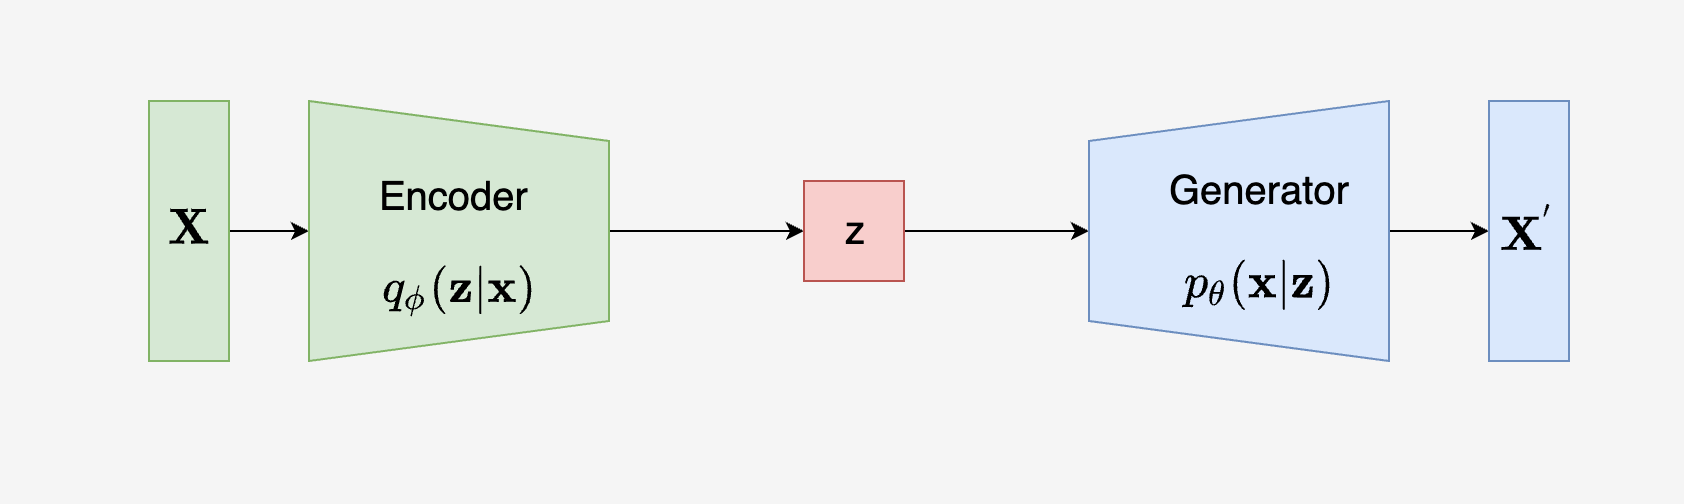
\includegraphics[width=0.9\textwidth]{./Images/VAE_structure.jpg}
    \caption{VAE structure showing the encoder and decoder processes.}
    \label{fig:VAE_structure}
\end{figure}


\subsubsection{VAE Loss Function}
The loss function of a VAE combines reconstruction loss with a Kullback-Leibler (KL) divergence term, which regularizes the latent space and encourages the model to learn a smooth and continuous representation \citep{10.3390/jimaging4020036}.

VAEs are trained to maximize the variational lower bound, which balances the accuracy of the reconstruction and ensures that the latent space is smooth and continuous. This allows the model to generate new data by sampling from the learned latent space and reconstructing the data using the decoder.

The loss function of VAE is as follows:

\begin{equation}
\mathcal{L} = \mathbb{E}_{q_\phi(z|x)}[\log p_\theta(x|z)] - D_{KL}(q_\phi(z|x) \| p(z))
\end{equation}

Where:
\begin{itemize}
    \item \(\mathcal{L}\): The total loss that the model aims to minimize.
    \item \(\mathbb{E}_{q_\phi(z|x)}[\log p_\theta(x|z)]\): The expected log-likelihood of reconstructing the data \(x'\) from the latent variable \(z\). The distribution \(q_\phi(z|x)\) represents the encoder, while \(p_\theta(x|z)\) represents the decoder's attempt to reconstruct the input data.
    \item \(D_{KL}(q_\phi(z|x) \| p(z))\): The Kullback-Leibler (KL) divergence, which measures the difference between the encoder's latent distribution \(q_\phi(z|x)\) and the prior distribution \(p(z)\), typically assumed to be Gaussian.
\end{itemize}

\subsection{Comparison with GANs}

In comparison to Generative Adversarial Networks (GANs), VAEs offer several key advantages. One of the primary benefits of VAEs is their simpler and more stable training process. GANs involve training two models simultaneously—a generator and a discriminator—which can result in unstable convergence and issues like mode collapse, where the generator fails to capture the diversity of the data. In contrast, VAEs have a single objective function that combines reconstruction loss and KL divergence, making the optimization process more straightforward \citep{10.1561/2200000056}.

Furthermore, the structured latent space of VAEs allows for meaningful interpolation between latent variables, enabling smooth transitions between generated data points. This makes VAEs particularly useful for tasks such as image generation, anomaly detection, and data imputation, where the ability to smoothly interpolate between data points is crucial \citep{10.1088/2632-2153/ab80b7}\citep{10.48550/arxiv.2002.10464}. GANs, on the other hand, do not explicitly model the latent space, which can limit their interpretability and ability to interpolate between generated samples.

However, GANs are known for producing sharper and more realistic images compared to VAEs, especially in high-resolution image generation tasks. This is because the adversarial loss in GANs encourages the generator to produce outputs that closely resemble real data, whereas VAEs tend to produce blurrier images due to the use of a Gaussian prior in the latent space \citep{10.1109/access.2020.2977671}. Despite this, VAEs are more flexible and scalable, as they can be trained with standard gradient descent methods and do not require the complex adversarial setup that GANs use.

\subsection{Applications of VAEs}

The structured latent space of VAEs not only allows for efficient sampling but also supports various applications. These include:
\begin{itemize}
    \item \textbf{Image Generation}: VAEs are capable of generating new images by sampling from the latent space and decoding them to the image space.
    \item \textbf{Anomaly Detection}: VAEs can identify outliers by measuring the reconstruction error, where high reconstruction loss may indicate anomalous data points.
    \item \textbf{Data Imputation}: VAEs can be used to fill in missing data by sampling from the latent space and reconstructing the missing portions of the data.
\end{itemize}

\subsection{Limitations of VAEs}

One notable limitation of VAEs is their difficulty in modeling discrete data. Since VAEs rely on backpropagation through continuous latent variables, handling discrete data types effectively poses a challenge \citep{10.48550/arxiv.1909.13062}. Additionally, the Gaussian assumption in the latent space can sometimes lead to less sharp or less diverse outputs compared to GANs. Despite these limitations, VAEs remain a powerful tool for representing high-dimensional complex data by learning a low-dimensional latent space in an unsupervised manner \citep{10.48550/arxiv.2106.06500}.


\section{Diffusion Models}

Diffusion models are the most recent advancement in generative models, first introduced in the early 2020s. These models take a different approach by progressively adding noise to data and then learning to reverse the process, effectively "denoising" the noisy data back into its original form.

The process involves two key steps, as shown in Figure~\ref{fig:Diffusion_structure}:
\begin{itemize}
  \item \textbf{Forward Process}: Gradually adds Gaussian noise to data \(x_0\), creating noisy versions of the data \(x_1, x_2, \dots, x_T\). Each step increases the level of noise, eventually leading to a completely noisy version \(z\).
  \item \textbf{Reverse Process}: The model learns to reverse the noise addition process, starting from the fully noisy version \(z\), and progressively denoising it to recover data that resembles the original input \(x_0\).
\end{itemize}

\begin{figure}[]
    \centering
    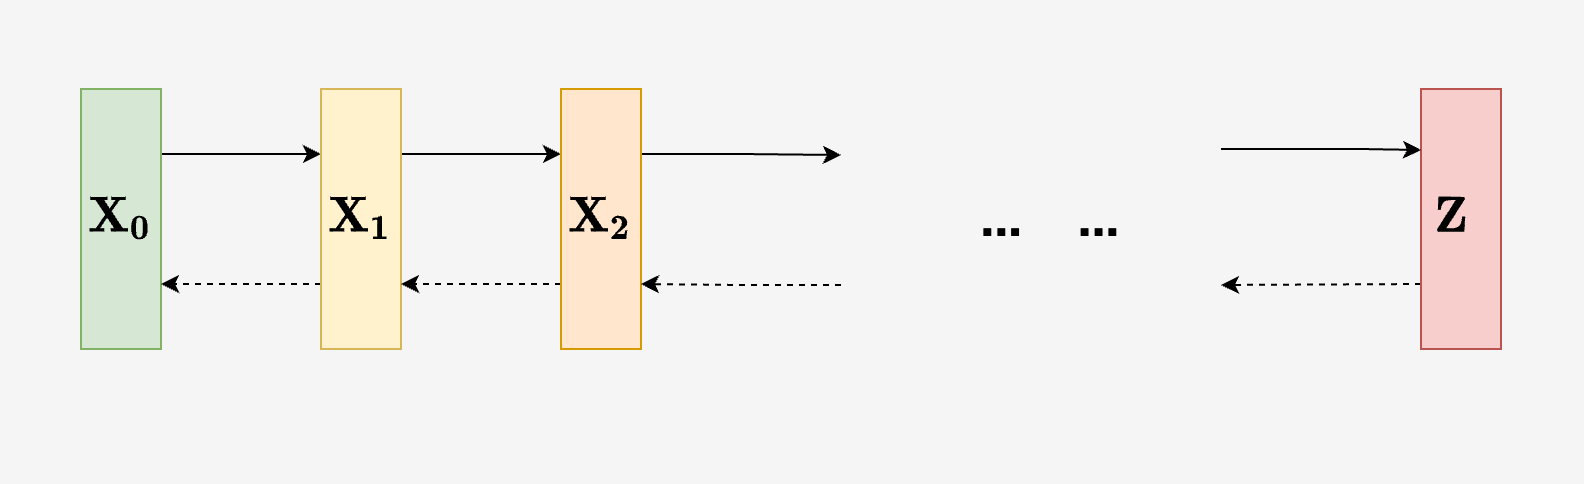
\includegraphics[width=0.9\textwidth]{./Images/Diffusion_structure.jpg}
    \caption{Diffusion model structure showing the forward and reverse processes.}
    \label{fig:Diffusion_structure}
\end{figure}

\subsection{Forward Process}
In the forward process, starting from the original data \(x_0\), Gaussian noise is added step-by-step to generate increasingly noisy versions of the data. Mathematically, the forward process is described as:

\begin{equation}
q(x_t | x_{t-1}) = \mathcal{N}(x_t; \sqrt{\alpha_t} x_{t-1}, \beta_t I)
\end{equation}

Where:
\begin{itemize}
    \item \(x_0\), \(x_1\), \(x_2\), \dots, \(x_T\): The sequence of noisy data at each time step.
    \item \(\alpha_t\): The scaling factor applied to the data at each step.
    \item \(\beta_t\): The variance of the Gaussian noise added at each step \(t\).
    \item \(\mathcal{N}(x; \mu, \sigma^2)\): A Gaussian distribution with mean \(\mu\) and variance \(\sigma^2\).
\end{itemize}

The process continues until we reach the final state \(z\), which is almost entirely noise.

\subsection{Reverse Process}
Once the noisy data is generated, the reverse process begins. The model learns to reverse the noise addition process to gradually recover the original data. The reverse process is defined as:

\begin{equation}
p_\theta(x_{t-1} | x_t) = \mathcal{N}(x_{t-1}; \mu_\theta(x_t, t), \Sigma_\theta(x_t, t))
\end{equation}

Where:
\begin{itemize}
    \item \(x_t\): The noisy data at time step \(t\).
    \item \(\mu_\theta(x_t, t)\): The model's predicted mean at step \(t\), parameterized by \(\theta\).
    \item \(\Sigma_\theta(x_t, t)\): The model's predicted variance at step \(t\), parameterized by \(\theta\).
    \item \(\mathcal{N}(x; \mu, \sigma^2)\): A Gaussian distribution with mean \(\mu\) and variance \(\sigma^2\).
\end{itemize}

The reverse process progressively reduces the noise added in the forward process, resulting in data that closely resembles the original input.

\subsection{Loss Function}
The training objective for diffusion models is to minimize the difference between the real data distribution and the distribution of generated data across all time steps:

\begin{equation}
L = \sum_{t=1}^{T} \mathbb{E}_{x_0, \epsilon} [\|\epsilon - \epsilon_\theta(x_t, t)\|^2]
\end{equation}

Where:
\begin{itemize}
    \item \(L\): The loss function to be minimized.
    \item \(T\): The total number of time steps in the diffusion process.
    \item \(x_0\): The original data sample.
    \item \(x_t\): The data at time step \(t\), after adding noise.
    \item \(\epsilon\): The noise added to the data at each step.
    \item \(\epsilon_\theta(x_t, t)\): The model's estimate of the noise at time step \(t\).
\end{itemize}

\subsection{Comparison with GANs}

Diffusion models differ significantly from Generative Adversarial Networks (GANs) in both training dynamics and generated data quality. One of the key advantages of diffusion models is their training stability. While GANs often suffer from issues like mode collapse and unstable training due to the adversarial nature of training two competing networks (generator and discriminator), diffusion models employ a simpler training process by learning to reverse the noise addition without requiring a discriminator \citep{ho2020denoising}.

Furthermore, diffusion models can generate high-quality and diverse samples by progressively denoising data, allowing for more controlled sample generation. In contrast, GANs tend to generate sharper but sometimes less diverse images due to the tendency of the generator to overfit to certain modes of the data distribution. Diffusion models, by their nature, ensure a gradual reconstruction from noise, which can avoid some of the issues of GANs \citep{nichol2021improved}.

However, GANs are often preferred for tasks requiring very sharp and realistic images, especially in high-resolution image synthesis. Diffusion models, while generally producing realistic images, may not always match the sharpness achieved by GANs in certain domains, particularly in tasks like photorealistic image generation.

\subsection{Applications of Diffusion Models}

Diffusion models have found a wide range of applications, especially in fields where stability and quality of generation are important. Some notable applications include:
\begin{itemize}
    \item \textbf{Image Generation}: Diffusion models have proven effective in generating photorealistic images, similar to GANs, but with more stable training dynamics.
    \item \textbf{Text-to-Image Generation}: Recent advancements have applied diffusion models to text-to-image synthesis, where a text prompt is converted into a corresponding image. These models can produce diverse outputs based on input descriptions.
    \item \textbf{Speech Synthesis}: Diffusion models have also been applied to generating high-quality audio data. For example, they are used in text-to-speech systems to generate realistic human speech \citep{chen2020wavegrad}.
    \item \textbf{Anomaly Detection}: Similar to VAEs, diffusion models can be used to detect anomalies by evaluating how well a noisy sample can be denoised. Poor reconstructions may indicate that the input is anomalous or different from the training data.
\end{itemize}

\subsection{Limitations of Diffusion Models}

Despite their advantages, diffusion models have several limitations:
\begin{itemize}
    \item \textbf{Computationally Intensive}: One of the primary drawbacks of diffusion models is that they are computationally expensive. The iterative process of adding and removing noise requires significantly more computation compared to GANs, which generate data in a single forward pass through the generator \citep{ho2020denoising}.
    \item \textbf{Generation Speed}: Diffusion models are slower than GANs in terms of sample generation. Since the process involves multiple time steps (often hundreds or even thousands), generating a single sample can take much longer compared to GANs, which generate samples almost instantaneously.
    \item \textbf{Sample Sharpness}: Although diffusion models tend to produce more diverse outputs compared to GANs, the sharpness of the generated images may not always match the high-quality, photorealistic outputs that GANs can achieve, especially in tasks that require very fine details.
\end{itemize}

